\documentclass{article}

\usepackage[final]{neurips_2018}
\usepackage[utf8]{inputenc} % allow utf-8 input
\usepackage[T1]{fontenc}    % use 8-bit T1 fonts
%\usepackage{hyperref}       % hyperlinks

\usepackage{url}            % simple URL typesetting
\usepackage{booktabs}       % professional-quality tables
\usepackage{amsfonts}       % blackboard math symbols
\usepackage{nicefrac}       % compact symbols for 1/2, etc.
\usepackage{microtype}      % microtypography
\usepackage{pifont}

%% RN stylefile
\usepackage{color,soul,upgreek}
\usepackage{arydshln}
\usepackage{wrapfig}
\usepackage{soul}
\usepackage{amsmath}
\usepackage{empheq}
\usepackage{enumerate}
\usepackage{morenotations,rotating}
\usepackage{color,soul,upgreek}
\usepackage{graphicx,caption,subcaption}
\graphicspath{{./Figs/}}

%\usepackage{xr-hyper} \externaldocument{nips18-coda-supp}

%% Tikz Support
\usepackage{tikz, pgfplots}
\usetikzlibrary{intersections, calc, positioning, decorations.pathreplacing}
\pgfplotsset{compat=1.8, xlabel style={anchor=west, align=center}, ylabel style={anchor=south, align=center}, samples=200, ymin=0, ymax=1, width=3cm, height=3cm, axis lines=middle, xticklabel style={/pgf/number format/.cd,frac,frac TeX=\frac}, yticklabel style={/pgf/number format/.cd,frac,frac TeX=\frac}, xtick=\empty,ytick=\empty, no markers, cycle list={{black,solid}}, samples=200}

\usepackage{color,soul}

\newcommand\MAF[1]{{\bf\color{magenta}{#1}}}

\bibliographystyle{plain}

\mdfdefinestyle{MyFrame}{%
  linecolor=gray,
  outerlinewidth=0.5pt,
  roundcorner=2pt,
  innertopmargin=4pt,
  innerbottommargin=4pt,
  innerrightmargin=4pt,
  innerleftmargin=4pt,
  leftmargin=0pt,
  rightmargin=0pt
}

\usepackage[toc,page,header]{appendix}
\usepackage{minitoc}
\renewcommand \thepart{}
\renewcommand \partname{}

\title{\papertitle} %New approaches to clustering directional statistics

\author{Marta Avalos-Fernandez$^\dagger$~~Richard Nock$^\ddagger$$^\S$$^\natural$~~Cheng Soon Ong$^\ddagger$$^\S$~~Julien Rouar$^\dagger$~~Ke Sun$^\ddagger$
\thanks{Authors in alphabetical order}\\
  $^\dagger$Universit\'e de Bordeaux,~~$^\ddagger$Data61,\\
  $^\S$the Australian National University and $^\natural$the University of Sydney\\
  \texttt{first.last@\{u-bordeaux.fr,data61.csiro.au\}}}
\date{\empty}

\begin{document}

\maketitle

\doparttoc % Tell to minitoc to generate a toc for the parts
\faketableofcontents % Run a fake tableofcontents command for the partocs

\begin{abstract}
  We consider the problem of learning a low dimensional representation for
  compositional data. Compositional data consists of a collection of nonnegative data
  that sum to a constant value. Since the parts of the collection are statistically
  dependent, many standard tools cannot be directly applied. Instead, compositional data must
  be first transformed before analysis. Focusing on
  principal component analysis (PCA), we propose an approach that allows low dimensional
  representation learning directly from the original data.
  Our approach combines the benefits of the log-ratio transformation from compositional
  data analysis and exponential family PCA.
  A key tool in its derivation is a generalization of the scaled Bregman
  theorem, that relates the perspective transform of a Bregman
  divergence to the Bregman divergence of a perspective transform and
  a \textit{remainder} conformal divergence.
  Our proposed approach includes a convenient surrogate (upper bound) loss of
  the exponential family PCA which
  has an easy to optimize form.
  We also derive the corresponding
  form for nonlinear autoencoders. Experiments on simulated data and microbiome data show
  the promise of our method.
\end{abstract}

\section{Introduction}

Compositional data analysis (CoDA)
is a subfield of statistics introduced more than three decades ago \cite{aTSB,aPCA,aTSJ,pbCD}.
Compositional data consist of a collection of nonnegative measurements that sum to a constant value, typically, proportions that sum to 1.
Because knowing the sum, one component can be determined from the sum of the remainder, the parts that make up the composition are mathematically and statistically dependent.
This distinct structure complicates analysis and does not allow standard statistical analyses. Ignoring the underlying nature of the data studied might give rise to misleading conclusions.
%CoDA is a subfield of statistics introduced more than three decades ago \cite{aTSB,aTSJ,pbCD}, in which data is subject to
%distinctive transformations (design principles) to satisfy some quite singular
%properties --- scaling, perturbation and permutation invariance,
%subcompositional coherence among others \cite{vtAC}. There is a stress to
%understand the soundness of models \cite{aeCD}.

Among others, \cite{aTSJ} and \cite{epmbIL} provided a framework to perform CoDA
by mapping data from the constrained simplex space to the Euclidian space using nonlinear log-ratio transforms.
In this paper, we focus on Principal Components Analysis (PCA),
one of the main tools for exploratory analysis of compositional data.
Just like in standard Euclidean data, it is particularly useful when the first few principal components explain enough variability to be considered as representative.
Unfortunately, any operation of centering or scaling destroys the compositional nature of
the data, which complicates a direct application of PCA.

Our motivation for studying CoDA comes from the recent
explosion of microbiome studies \cite{grCAA, gwpeIAR}.
Indeed, spectacular advances in 16S rRNA gene sequencing of the bacterial component of the human microbial community (microbiota) have enabled researchers to investigate human health and disease, leading to new insights into the role of these microbial communities.
The microbiota sequencing data are measured as read counts interpreted as a species' abundance in a microbial community. To make the microbial abundance comparable across samples, data are normalized to the relative abundances of all bacteria observed.
On the other hand, because high-throughput experiments produce large amounts of data, multivariate analysis is indispensable \cite{psAMS,haAMCC}.
There is a stress to understand the soundness of models \cite{aeCD}.
%The use of a more natural measure for CoDA may optimize the projection and visualization with respect to log-ratio transformed PCAs.

In this paper, we propose to learn a low dimensional representation of CoDA from the
\emph{original} data. To account for the nonlinearity due to the compositional nature
of the data, we start from exponential family PCA~\cite{cdsAG} that we
augment with the compositional constraint and then simplify the loss
to be optimized via a generalization of a recent result~\cite{nmoAS}
on Bregman divergences, which may be of independent interest.
We also propose a nonlinear
autoencoder (AE) version to learn the low dimensional representation.

\begin{figure}[t]
\centering
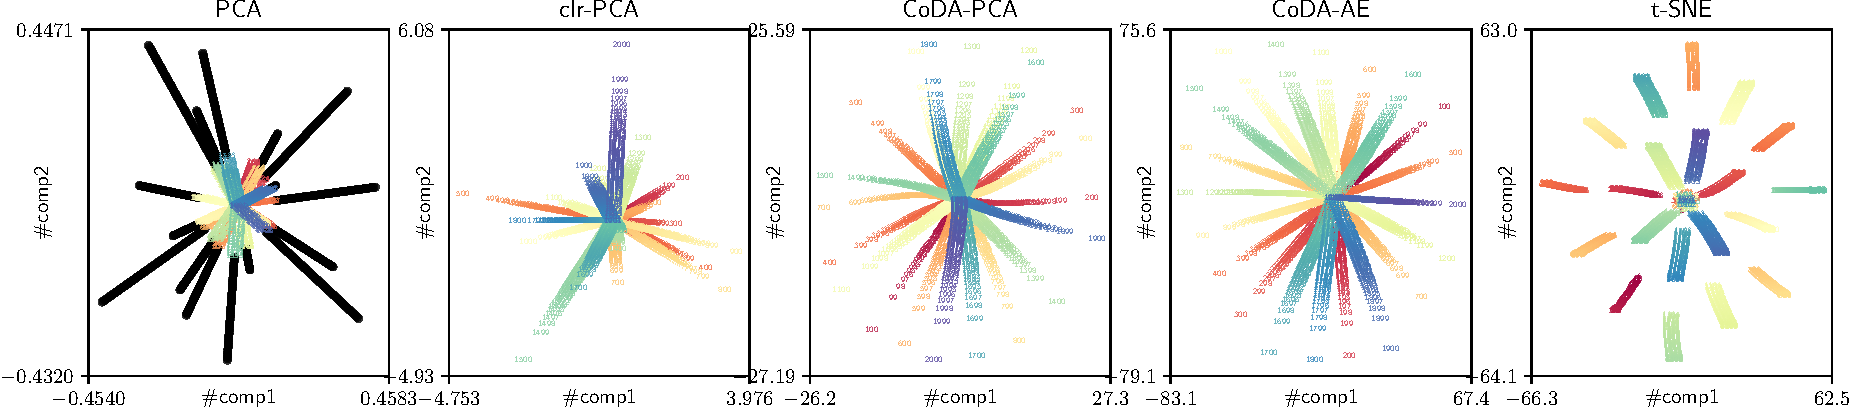
\includegraphics[width=\textwidth]{20arms_scatter.pdf}
\caption{2D Visualization of the low dimensional representation $\A$ on the \texttt{arms} dataset.}\label{fig:arms}
\end{figure}

Let us examine a toy example to illustrate our approach.
We generate the \texttt{arms} dataset in $\Se^{19}$
by evenly interpolating the simplex center and each of the 20 vertices with 100 points,
therefore yielding a matrix $\X_{20\times2000}$.
Figure~\ref{fig:arms} shows the 2D representation
$\A_{2\times2000}$ computed by five methods:
the standard \texttt{PCA};
\texttt{clr-PCA} computes the standard PCA after performing clr;
\texttt{CoDA-PCA} and \texttt{CoDA-AE} are our proposed methods;
t-SNE~\cite{maaten08} is a popular nonlinear dimensionality reduction
method and is applied on $\X$ directly.
In the \texttt{PCA} plot, the black segments indicate that
the PCA reconstruction is outside of the simplex. PCA cannot be directly adapted to CoDA
because the projection on the principal components may go beyond the convex hull of the vertices.
It is clear that only \texttt{CoDA-PCA} and \texttt{CoDA-AE} uncover
the true structure,
where all the arms are clearly presented, and their connections are faithfully presented.

\section{Compositional Data Analysis}

We briefly review some definitions of CoDA.
Compositional data are proportions: $\X$ is a compositional dataset if and only if
$\X\in\Re^{d\times m}$ such that $\forall{i}\in [1,...,m]$ the vector column
$\ve{x}_i$ of $\X$ is in the simplex
$\Se^d=\big\{\ve{x}\in\Re^d\,:\,\forall{j}, x_j> 0;\:\sum_{j=1}^d{x}_j=\kappa\big\}$,
where $\kappa>0$ is a constant, classically $1$.
Here the superscript $d$ does not denote the dimensionality as $\dim(\Se^d)=d-1$.
For a dataset $\X'$ which contains counts of strictly positive values,
we reduce it to a compositional dataset by dividing out the totals, that is
we compute the CoDA set $\X$ such that:
$\ve{x}_i=\ve{x'}_i\frac{1}{\sum_{j=1}^dx'_{ji}}$
is the vector of proportions for individual $i$.

Using Bregman divergences makes explicit a dual affine~\cite{aIG}
coordinate space which is in fact the log coordinates of Aitchison~\cite{aTSJ}.
It is in this space that we have affine constraints, which are therefore non-linear
in the "primal", ambient space.
To manage this nonlinear structure,
it has been proposed~\cite{aPO} to first apply a log-ratio transformation to transpose the data into real Euclidean space. For instance, the additive log-ratio transformation (alr) applies log-ratio between a component and a reference component; the centered log-ratio transformation (clr) scales each subject vector by its geometric mean; and the isometric log-ratio transformation (ilr) is associated with an orthogonal coordinate system in the simplex.
Afterwards, standard PCA is performed.

By definition, the clr transformation is
\begin{equation}\label{eq:clr}
\clrlog(\ve{x})
= \log\left(\frac{\ve{x}}{g(\ve{x})}\right)
= \C^{\mathrm{clr}} \log(\ve{x})
= \log(\ve{x})-\overline{\log(\ve{x})}\bm{1}_d,
\end{equation}
where $g(\ve{x})=(\prod_{j=1}^d x_j)^{1/d}$ the geometric mean of $\ve{x}$,
$\overline{\ve{x}}=\frac{1}{d}\sum_{j=1}^d x_j$ is the arithmetic mean of $\ve{x}$,
$\bm{1}_d$ is the $1\times{d}$ vector of all ones,
and $\C^{\mathrm{clr}}=\I_{d}-\frac{1}{d}\bm{1}_d\bm{1}_d^\top$.
The purpose of the log-ratio transformation (centered or not) is to go back to $\Re^d$ from $\Se^{d}$ without losing information.
Notice that $\log(x_{j})$, $\overline{\log(\ve{x})}\in(-\infty,0)$ so the compositional data is embedded in $\Re^d$ under the clr transformation.
The reverse operation:
$\ve{x}=\clrlog^{-1}(\ve{x'})=\exp(\ve{x'})\prod_{j=1}^d \exp(\frac{1}{1-d}x'_{j})$ embeds $\Re^d$ into $\Se^{d}$.
See the table below for a comparison of clr, alr and ilr, presented
as different transformations $\C\log(\bm{x})$.
They are equivalent up to linear transformations.
Without loss of generality we focus on the clr.

\begin{center}
  \begin{tabular}{c||c||c}
  \toprule
  clr & alr & ilr \\
  \hline
  $\C^{\mathrm{clr}}_{d\times{d}}=\I_{d}-\frac{1}{d}\bm{1}_d\bm{1}_d^\top$
  & $\C^{\mathrm{alr}}_{(d-1)\times{d}}=\left[\I_{d-1},-\bm{1}_{d-1}\right]$
  & $\C^{\mathrm{ilr}}_{(d-1)\times{d}}\in\left\{\R\C^{\mathrm{clr}}\,:\,\R\R^\top=\I_{d-1}\right\}$ \\
  \bottomrule
  \end{tabular}
\end{center}

%Any operation of centering or scaling will erase the CoDA or counting nature of the data, it's not a costless operation.
%With the centered log-ratio operation, Aitchison brought a solution to this problem.

%Results could then be visually represented in the 2-dimensional Euclidian space: log-ratio transformed data points and vectors of the original basis are expressed on the basis of the principal coordinates. Occasionally, the first principal components are back-transformed and represented in the 2-dimensional ternary diagram, an equilateral triangle whose vertices represent the three elements of a 3-part composition or two of the elements and the addition of the other $d-2$ elements of a $d$-part composition.

%Simply log-transforming the CoDA allows applying standard multivariate analysis techniques.
However interpreting the resulting coordinates is still challenging \cite{epmbIL, mpetTS}:
alr transformation is no distance-preserving;
%(it is an isomorphism, but not an isometry);
clr leads to degenerate distributions and singular covariance matrices;
%(it is an isometry but between the simplex and a subspace of the Euclidian space of the same dimension);
ilr avoids the precedent drawbacks,
%(it is an isometry between the simplex and a subspace of the Euclidian space of the same dimension minus one),
but still, results from complicated nonlinear transformations are difficult to interpret.
Currently, there seems to be no consensus about the best practices (\cite{gCDAP} versus \cite{petLNCDA}) and, in all cases, log-transforming is not a remedy for all the difficulties arisen by CoDA \cite{lmtzhCCC}.

\section{Exponential Family Principal Component Analysis}

Another way to apply dimension reduction is to perform a generalized PCA on crude count data.
Based on the same ideas as the generalised linear model, \cite{cdsAG} described a
generalized PCA model for distributions from the exponential family.
We first recall the standard PCA setting.

\subsection{Principal Component Analysis}

For simplicity suppose that the data matrix $\X$ is already centered
that can be easily achieved by appending to $\A$ matrix a row of ones.
\begin{mdframed}[style=MyFrame]
(Traditional PCA) We have a dataset $\X \in \Re^{d \times m}$ that we approximate as
$\X \sim \V^\top \A$ by minimizing the following loss wrt the constraints
$\A \in \Re^{\ell \times m}\:,\:\V \in \Re^{\ell \times d}\:,\:\V \V^\top = \I_\ell$:
\begin{equation}
\ell_{\mathrm{PCA}}(\X; \A,\V) \defeq \|\X - \V^\top \A\|_\mathrm{F}^2\:\:.\label{defSQL}
\end{equation}
\end{mdframed}
Hence, observations are column-wise. $\V : \Re^d \rightarrow
\Re^\ell$ is surjective with $\V^\top \V$ defining a rank-$\ell$
projection, assuming in general $\ell < d$. $\A$ is the representation
of data points. The goodness of fit of the
representation is measured by the squared Frobenious norm.
We summarise the different transformations and loss functions in
Table~\ref{tab:summary-of-methods}.

Observe that instead of finding a linear representation $\A$ and its corresponding
linear loadings $\V$, we can consider nonlinear functions for encoding and decoding
the latent representation. When the nonlinear encoder and decoder are implemented as
feed-forward neural networks, we arrive at the autoencoder setting.

\subsection{Bregman Divergence and $\varphi$-PCA}

As mentioned in the introduction, compositional data do not live in Euclidean space.
Count data are naturally linked to the Poisson distribution,
and therefore we should consider an exponential family model for count data.
From the Bayesian viewpoint,
the PCA goal is to minimize a distance ($L^2$ for usual PCA) which is equivalent
to a Bregman divergence minimization (or a Likelihood function maximization).

\begin{definition}[Bregman Divergence]\label{defBREG}
Let $\varphi : \Re^{d} \rightarrow \Re$
convex differentiable. The Bregman divergence $D_\varphi$ with
generator $\varphi$ is
\begin{equation}
D_\varphi(\ve{x}\,\Vert\,\ve{x}') \defeq \varphi(\ve{x}) -
\varphi(\ve{x}') - (\ve{x}-\ve{x}')^\top\nabla\varphi(\ve{x}').
\end{equation}
\end{definition}
A Bregman divergence is just a truncation of the Taylor expansion of a
function. It can therefore be defined for any differentiable function,
not just the convex ones. If $\varphi$ is \textit{not} convex, we
call $D_\varphi$ a \textit{Bregman distortion}, which is a signed dissimilarity.
We denote by
$\varphi^\star(\ve{x}) \defeq \sup_{\ve{y}} \{\ve{x}^\top \ve{y} - \varphi(\ve{y})\}$
the convex conjugate of the generator $\varphi$~\cite{bvCO}.

PCA has been generalized to the exponential families in a way that
makes fitting occur in the \textit{natural parameter} space \cite{cdsAG,lGPCA}
(and references therein).
The optimization problem is non-convex.
The algorithmic strategy proposed by \cite{cdsAG} is to use
an alternating sequence of convex minimizations under constraints.
Alternatively, \cite{lGPCA} proposed maximizing the deviance (as a generalized notion of variance) and \cite{cmrVI} proposed
maximizing the likelihood function via a variational algorithm and gradient descent.

We denote exponential family PCA as $\varphi$-PCA, where $\varphi$
is the cumulant of the exponential family, which
is strictly convex differentiable with convex conjugate $\varphi^\star$,
and uniquely determines the exponential family under mild conditions \cite{bIA}.
Note that for $\varphi$-PCA, $\X$ is not neccessarily in a vector space
(e.g. $\X\not\subseteq\Re^{d\times m}$).
\begin{mdframed}[style=MyFrame]
($\varphi$-PCA) We have a dataset $\X_{d\times m}$ that we approximate as
$\X \sim \nabla\varphi^\star (\V^\top \A)$
with $\A\in\Re^{\ell\times m}$, $\V\in\Re^{\ell \times d}$, $\V\V^\top = \I_\ell$,
through minimizing the Bregman loss
\begin{equation}
\ell_{\varphi\text{-}\mathrm{PCA}}(\X; \A, \V)
\defeq
\sum_i D_\varphi(\ve{x}_i\,\Vert\,\nabla\varphi^\star(\V^\top \ve{a}_i))
=
D_\varphi(\X\,\Vert\,\nabla\varphi^\star(\V^\top \A)).\label{eqEXP-PCA}
\end{equation}
\end{mdframed}
Vectors are column-vectors: $\ve{x}_i, \ve{a}_i$
are respectively column observation $i$ in the ambient and principal spaces, respectively.
This formulation has a major advantage that linear algebra may be
used to fit $\A, \V$ while $\X$ may not lie in a vector space, see
for example \cite{cdsAG,lGPCA} and references therein.
We remark that because
of the dual symmetry of Bregman divergences, we have
$D_\varphi(\X\,\Vert\,\nabla\varphi^\star(\V^\top\A))
= D_{\varphi^\star}(\V^\top\A\,\Vert\,\nabla\varphi(\X))$ \cite{bnnBV}.
Notice there exists a little "hole" in the
$\varphi$-PCA definition, as $\X$ is not necessarily easy to center
when it is not in a vector space.

$\varphi$-PCA includes standard PCA as a special case as when $\varphi(\bm{x})=\frac{1}{2}\Vert\bm{x}\Vert_{\mathrm{F}}^2$ and
the corresponding Bregman divergence becomes $D_\varphi(\bm{x}\,\Vert\,\bm{x}')=\frac{1}{2}\Vert\bm{x}-\bm{x}'\Vert_{\mathrm{F}}^2\:$.

\section{Exponential family PCA on Compositional Data}

\begin{table}[t]
  \caption{Summary of methods in this paper}
  \begin{tabular}{l||c|c|c||l}
    \toprule
    Method&Original&Reconstruction&Distortion&Notes\\
    \hline
    PCA&$\X$ &$\V^\top \A$&$\|\cdot - \cdot\|_\mathrm{F}^2$
    &classical PCA\eqref{defSQL}\\
    $\varphi$-PCA & $\X$& $\nabla^*\varphi(\V^\top \A)$ & $D_\varphi(\cdot\,\Vert\,\cdot)$
    & exponential family PCA \eqref{eqEXP-PCA}\\
    clr-PCA& $\clrlog(\X)$ &$\V^\top \A$&$\|\cdot - \cdot \|_\mathrm{F}^2$
    & CoDA with clr \eqref{coda-pca}\\
    gauged-$\varphi$-PCA&$\nabla\varphi(\check{\X})$&$\V^\top \A$ &$D_{\varphi^\star}(\cdot\,\Vert\,\cdot)$
    &General Bregman PCA \eqref{eqEXP-PCA-DUAL-GAUGED}\\
    CoDA PCA&$\clrlog({\X})$&$\V^\top \A$&$D_{\exp}(\cdot\,\Vert\,\cdot)$
    &\eqref{pb-CoDA} is a special case of  \eqref{eqEXP-PCA-DUAL-GAUGED}\\
    $\surrogateCoDAPCA$&$\check{\ve{x}}_i$&$\nabla \check{\kl}(\exp(\V^\top \ve{a}_i))$&
    inner product&upper bound \eqref{pb-s-CoDA}\\
    CoDA AE&$\X$&$g_\theta \circ h_\Phi(\X)$&$D_{\exp}(\cdot\,\Vert\,\cdot)$
    &neural networks $g_\theta$ and $h_\Phi$\\
    \bottomrule
  \end{tabular}
  \label{tab:summary-of-methods}
\end{table}

CoDA has
found a workaround for the centering problem, \textit{centered log-ratio
 coordinates}.
From \cite[Def. 4.6, Chap. 8]{aTSB} the associated loss is
the standard PCA loss on clr transformed data:
\begin{equation}
\ell_{\mathrm{clr\text{-}PCA}}(\X; \A,\V)
\:\defeq\:\frac{1}{2}\|\clrlog(\X) -\V^\top \A\|_\mathrm{F}^2\label{coda-pca}
\:=\: D_\varphi(\clrlog(\X)\,\Vert\,\nabla\varphi^\star(\V^\top \A)),
\end{equation}
where $\clrlog(\X)$ is the centered log-ratio transform defined in
Equation~\eqref{eq:clr} and $\varphi(\bm{x})=\frac{1}{2}\Vert\bm{x}\Vert_{\mathrm{F}}^2$.
Recall from the previous section that we could deal with crude count data by using
exponential family PCA.
However if we wish to perform PCA on the crude count data, while maintaining the clr transform,
we need an additional normalization
term, which requires us to obtain a gauged version of the Bregman divergence.

\subsection{Scaled Bregman Theorem with Remainder}

In this section we generalize the Scaled Bregman Theorem from \cite[Theorem 1]{nmoAS}
to allow for a remainder term.
We use it in this paper to deal with the perspective transform required for CoDA,
but it may be of independent interest. Recall that $\varphi$ is the generator
of the Bregman distortion (Definition~\ref{defBREG}). We additionally define
a perspective (or gauge) function $g$ to deal with the fact that we are considering
data on the simplex.
Whenever $\varphi$ and $g$ are differentiable, the following is
immediate from \cite[Theorem 1]{nmoAS}.
\begin{mdframed}[style=MyFrame]
\begin{theorem}[Scaled Bregman Theorem with Remainder]\label{th00}
For any
$\varphi: \XCal \rightarrow \Re$ and $g : \XCal \rightarrow \Re_*$ ($\Re_*=\Re\setminus\{0\}$)
that are both differentiable, denoting
\begin{equation}
  \check{\ve{x}} \defeq \frac{\ve{x}}{g(\ve{x})}
  \quad\text{and}\quad
  \check{\varphi}(\ve{x}) \defeq
  %g(\ve{x}) \cdot {\varphi}(\check{\ve{x}})  =
  g(\ve{x}) \cdot {\varphi}\left( \frac{\ve{x}}{g(\ve{x})} \right) \:\:,\label{defCHECKPHI}
\end{equation}
the following holds true:
  \begin{equation}
  g(\ve{x}) \cdot D_{\varphi}\left( \vexdagger \,\Vert\, \veydagger \right)
  = D_{\varphidagger}\left( \ve{x} \,\Vert\, \ve{y}\right)
  + R_{\varphi, g}(\ve{x}\,\Vert\,\ve{y})\:,\quad\forall
  \ve{x}, \ve{y}\in \XCal\:\:,\label{defdagger}
  \end{equation}
  where $R_{\varphi, g}(\ve{x}\,\Vert\,\ve{y}) \defeq \varphi^\star\left(\nabla\varphi(\veydagger)
  \right)\cdot D_g(\ve{x}\,\Vert\,\ve{y})$ is called the \emph{remainder}.
\end{theorem}
\end{mdframed}
We can abstract Theorem \ref{th00} by saying that for any $\varphi, g$
differentiable, we have
%\begin{mdframed}[style=MyFrame]
\begin{equation*}
\mathrm{perspective\text{-}Bregman}(\varphi, g)
=
\mathrm{Bregman}(\mathrm{perspective}(\varphi))
+ \mathrm{conformal\text{-}Bregman}(g, \varphi),
\end{equation*}
%\end{mdframed} % only use frame for PCA variants
where
``$\mathrm{perspective}(\varphi)$'' is $\check{\varphi}$ in \eqref{defCHECKPHI},
and conformal divergences are defined and analyzed in
\cite{nnaOCD}. General classes of perspective transforms of convex
functions are introduced in \cite{mOAI,mOAII}. The notion of
perspective transform of a Bregman divergence was introduced in \cite{nmoAS}.
In \cite[Theorem 1]{nmoAS}, conditions are assumed that make $R_{\varphi, g}(\ve{x}\,\Vert\,\ve{y}) = 0$,
resulting in the scaled Bregman theorem. Notice that
$D_\varphi$ is a Bregman distortion but not necessarily a Bregman divergence
if $\varphi$ is not convex. For reasons explained in \cite{nmoAS},
we call $g$ a \emph{gauge}. In the following we assume that $\varphi$ is
separable, so that we can use both notations $\nabla\varphi$ and
$\varphi'$ to denote the gradient and derivatives involving $\varphi$.

By Theorem~\ref{th00}, as long as $g(\ve{x})$ is homogeneous of degree one,
$D_{\varphi}\left( \vexdagger \,\Vert\, \veydagger \right)$ and
$\frac{1}{g(\ve{x})} \left[D_{\varphidagger}\left( \ve{x} \,\Vert\, \ve{y}\right) + R_{\varphi, g}(\ve{x}\,\Vert\,\ve{y})\right]$
are both invariant to re-scaling of $\ve{x}$ and $\ve{y}$ and can therefore be used to deal with compositional data.
A general formulation of $g$ satisfying this condition can be
$g(\ve{x})=\prod_{j=1}^d x_j^{w_j}$, where $\forall{j}, w_j\ge0$ and $\sum_{j=1}^d w_j=1$.
In this paper, we focus on the special case $\forall{j}$, $w_j=\frac{1}{d}$ so that
$D_{\varphi}\left( \vexdagger \,\Vert\, \veydagger \right)$
can be expressed in terms of the widely used clr transformation.
Setting $\bm{w}$ to be a one-hot vector $(1,0,\cdots,0)$ can
express $D_{\varphi}\left( \vexdagger \,\Vert\, \veydagger \right)$
with the alr. This latter case will be omitted here.

\subsection{Exponential Family CoDA}

We are now in a position to derive the exponential family version of the loss in \eqref{coda-pca}.
Let %$\check{\ve{x}} \defeq (1/g(\ve{x})) \cdot \ve{x}$ and define the corresponding matrix
$\check{\X}$ denote the matrix of the column vectors $\check{\ve{x}}_i$.
It turns out that in the same way as \eqref{defSQL} is an
approximation of \eqref{eqEXP-PCA}, the loss in \eqref{coda-pca}
is an approximation of the gauged loss:
\begin{equation}
\ell_{\mathrm{gauged\text{-}\varphi\text{-}PCA}}(\X; \A, \V) \defeq
D_{\varphi^\star}(\V^\top \A\,\Vert\,\nabla\varphi(\check{\X}))\label{eqEXP-PCA-DUAL-GAUGED}
\:=\:
D_{\varphi}(\check{\X}\,\Vert\,\nabla\varphi^\star(\V^\top\A)).
\end{equation}
Note that the above expression is in terms of the normalised matrix $\check{\X}$.
To unpack it in terms of the original data $\X$, we apply Theorem~\ref{th00}.
In the CoDA case, $\varphi^\star(z) \defeq \exp z$, the convex dual of
$\varphi(z) \defeq z \log z - z$. Indeed, after remarking that
$\nabla\varphi(\check{\X}) = \clrlog({\X})$, it follows
\begin{align}
\ell_{\mathrm{gauged\text{-}\kl\text{-}PCA}}(\X; \A, \V)
&=
D_{\exp}(\V^\top \A\,\Vert\,\clrlog({\X}))\label{eqEXP-PCA-DUAL2}
=
D_{\kl}\left(\check{\X}\,\Vert\,\exp(\V^\top \A)\right)\nonumber\\
&=
\bm{1}^\top\exp(\V^\top\A)\bm{1} - \mathsf{trace}\left(\check{\X}^\top \V^\top \A\right)
+ \mathrm{constant}.
%\sim \ell_{\mathrm{clr\text{-}PCA}}(\X; \A,\V) \:\:.
\end{align}
In other words, the CoDA PCA is in fact fitting natural parameters
from centered log-ratios being natural coordinates as well.
From (\ref{eqEXP-PCA-DUAL2}) we observe that both of them live in the same space.
Therefore $\V^\top\A$ is centered in the same way as $\clrlog({\X})$, and so
\begin{eqnarray}
\V \ve{1}_d \in \mathrm{ker}(\A^\top) & \Leftrightarrow & \A^\top \V \ve{1} =  \ve{0}_m\:\:.\label{condAV1}
\end{eqnarray}
Remark that a centering assumption is also explicit in \cite[Chapter 8, Eq. 8.1]{aTSB}.
%Consider $\bm{x}\in\Se\cup\partial\Se$ may contain zero entries
%and let $\ICal^+=\vert\{j\,:\,x_j>0\}\vert$ be the set of positive indices.
%Denote $\Se_{\bm{x}}=\{\bm{y}\in\Se\cup\partial\Se\,:\,
%\forall{j}\in\ICal^+, y_j>0\}$ which properly contains a small neighbourhood of $\bm{x}$.
%We have the following basic property of $D_{\exp}(\V^\top \A\,\Vert\,\clrlog({\X}))$:
%\begin{proposition}\label{thmSMOOTH}
%$\forall\ve{x}\in\Se\cup\partial\Se$,
%$D_{\exp} (\ve{y}\,\Vert\,\clrlog(\ve{x}))$ is a smooth function
%(indefinitely differentiate) on the extended plane
%$ \left\{ \bm{y}\,:\,\bm{1}^\top\ve{y}=0;\,%
%-\infty\le{}y_j<\infty\text{ if }x_j=0;\,%
%-\infty<y_j<\infty\text{ if }x_j>0\right\}$
%where we allow certain elements of $\ve{y}$ to be $-\infty$ if the corresponding elements of $\ve{x}$ are 0.
%\end{proposition}
%In $\ell_{\mathrm{CoDA\text{-}PCA}}(\X; \A, \V)$, $\V^\top\A$ can be regarded as
%the clr transformation $\clrlog(\hat{\X})$, where $\hat{\X}$ is the \CoDAPCA~reconstruction of $\X$.
%Therefore, the loss function of \CoDAPCA~smoothly extends to the boundary
%$\partial\Se$ as well, where $\A$ can have infinite values, and one can have semi-differentiations (consider
%the one-side differentiation in calculus).
%This is in contrast to clr-PCA as in \eqref{coda-pca}, where the loss is only defined inside $\Se$.

%\begin{proposition}
%\forall{\V}, $\forall\check{\X}$,
%\min_{\A\in\Re^{\ell\times{}m}}
%\left[ \bm{1}^\top\exp(\V^\top\A)\bm{1} - \mathrm{trace}\left(\check{\X}^\top V^\top \A\right) \right] \le
%\end{proposition}

%\CoDAPCA~can naturally deal with small compositional components.

Hence, we can define the CoDA PCA problem as follows.
\begin{mdframed}[style=MyFrame,nobreak=True]
(CoDA PCA) We have a dataset $\X \in (\Se^{d})^m$ that we approximate as
$\clrlog(\X) \sim \V^\top \A$ by minimizing the following loss wrt the constraints
$\A \in \Re^{\ell \times m}\:,\:\V \in \Re^{\ell \times d}\:,\:\V \V^\top = \I_\ell\:,\:\A^\top\V\ve{1} = \ve{0}$:
\begin{equation}
\ell_{\mathrm{CoDA\text{-}PCA}}(\X; \A, \V)\label{pb-CoDA}
= D_{\exp}(\V^\top \A\,\Vert\,\clrlog({\X})).
\end{equation}
\end{mdframed}

Regarding $\clrlog(\bm{x})$, $\check{\bm{x}}$ and $\bm{x}$ as different coordinate systems of $\Se^d$,
we use the Fisher information metric (FIM)~\cite{aIG}, whose formulation is well studied on the $\bm{x}$ coordinates,
to define the corresponding \emph{pullback metric} $\mathcal{G}$ under the
$\clrlog(\bm{x})$ and $\check{\bm{x}}$ coordinates,
meaning that these metrics correspond to the same underlying geometry of $\Se^d$.
We have the following proposition (proof omitted; see \cite{smAI} for similar derivations).
\begin{proposition}
The FIM that uniquely defines the geometry of
$\bm{c}\in\left\{\clrlog(\bm{x})\,:\,\bm{x}\in\Se^d\right\}$ is given by
$\mathcal{G}_{ij}(\bm{c})=\delta_{ij} \frac{\exp(c_i)}{\sum_{i=1}^d\exp(c_i)} - \frac{\exp(c_i+c_j)}{\left(\sum_{i=1}^d\exp(c_i)\right)^2}$;
the FIM under the coordinates $\check{\bm{x}}$ is given by
$\mathcal{G}_{ij}(\check{\bm{x}})=\delta_{ij} \frac{1}{\check{x}_i\sum_{i=1}^d\check{x}_i} - \frac{1}{(\sum_{i=1}^d\check{x}_i)^2}$,
where $\delta_{ij}=1$ if $i=j$ otherwise $\delta_{ij}=0$.
\end{proposition}
Intuitively, the metric $\mathcal{G}$ measures the local distance
$\mathrm{d}\check{\bm{x}}^\top\mathcal{G}(\check{\bm{x}})\mathrm{d}\check{\bm{x}}^\top$
of a tiny shift $\mathrm{d}\check{\bm{x}}$. It is not everywhere identity as in a Euclidean space.
Therefore the distance should not be measured by the Frobenious norm as in \eqref{coda-pca}.
In contrast, our loss $\ell_{\mathrm{CoDA\text{-}PCA}}(\X; \A, \V)$
is based on the KL divergence which locally agrees with the FIM~\cite{aIG}.

\subsection{Relating CoDA PCA to $\varphi$-PCA}

We now define and analyze a generalized perspective transform of the
generator of KL divergence: let $\check{\kl}(\ve{x}) \defeq g(\ve{x}) \cdot \sum_{j=1}^d \varphi(x_j /
g(\ve{x}))$ where $\varphi(z) \defeq z\log(z) - z$ and
$g(\ve{x})\defeq (\prod_j x_j)^{1/d}$.
\begin{lemma}\label{lemHESS}(Properties of $\check{\kl}$)
$\check{\kl}$ satisfies the following properties:
\begin{itemize}
\item [(1)] $\check{\kl}$ is convex;
\item [(2)] the general term of the
Hessian $\hessian$ of $\check{\kl}$ is
\begin{eqnarray}
\hessian_{ij} \defeq \hessian_{ij}(\check{\kl}(\ve{x})) & = &
\frac{1}{dx_j} \cdot \left\{
\begin{array}{ccl}
-u_{ji} & \mbox{ if } & j\neq i\\
\sum_{k\neq j} u_{kj} & \multicolumn{2}{c}{\mbox{ otherwise }}
\end{array}
\right. ,
\end{eqnarray}
where $u_{ab} \defeq 1+ x_a/x_b$. Furthermore,
\begin{eqnarray}
\ve{z}^\top \hessian \ve{z} & = & \frac{1}{2d}\sum_{ij}(x_i+x_j)\cdot \left(\frac{z_i}{x_i}-\frac{z_j}{x_j}\right)^2, \forall \ve{z}\in \Re^d.
\end{eqnarray}
Hence, $\ve{z}^\top \hessian \ve{z} \geq 0, \forall \ve{x} \in
\Re_{++}^d, \forall \ve{z} \in
\Re^d$ and $\ve{z}^\top \hessian \ve{z} = 0$ only when
$\ve{z} \propto \ve{x}$;
\item [(3)] function $\check{\kl} \circ \exp$ is 1-homogeneous on
  $\mathrm{span}(\{\ve{1}\})^\bot$.
\end{itemize}
\end{lemma}
(Proof in \SM, Section \ref{sec-proof-lemHESS})
A consequence of Theorem \ref{th00} is the following Corollary.
\begin{corollary}\label{corCoDA}
For any $\A$, $\V$ such that $\A^\top \V \ve{1} = \ve{0}$, we have
\begin{eqnarray}
 \ell_{\mathrm{CoDA\text{-}PCA}}(\X; \A, \V)  & \leq &
 \tilde{\ell} \defeq \sum_i \frac{1}{g(\ve{x}_i)} \cdot D_{\check{\kl}} (\ve{x}_i \|
\exp(\V^\top \ve{a}_i)).\label{eqBOUND1}
\end{eqnarray}
Hence, the CoDA PCA loss is upperbounded by a weighted generalized
$\varphi$-PCA loss. Furthermore,
\begin{eqnarray}
D_{\check{\kl}} (\ve{x}_i \|
\exp(\V^\top \ve{a}_i)) & = & \check{\kl}(\ve{x}_i) - \ve{x}_i^\top \nabla \check{\kl}(\exp(\V^\top
   \ve{a}_i))\label{eqBOUND2}
\end{eqnarray}
\end{corollary}
\begin{proof}
Since $g$ is concave (Example \ref{exGEOM} in Supplement), $D_g(\ve{x}\|\ve{y}) = -
D_{-g}(\ve{x}\|\ve{y})\leq 0$, and \eqref{eqBOUND1} follows from
Theorem \ref{thCODA1} and the fact that $r_i\geq 0, \forall i$, which
shows \eqref{eqBOUND1}. \eqref{eqBOUND2} is a consequence of the
analytical construct of Bregman divergences (Definition \ref{defBREG}) and point (3)
in Lemma \ref{lemHESS}
 and the fact that $\V^\top
   \ve{a}_i \in \mathrm{span}(\{\ve{1}\})^\bot$ by assumption.
\end{proof}
\begin{remark}
In \cite[Chapter 8]{aTSB}, CoDA PCA is presented as a (centered)
regular PCA over data that been subject to \textit{two} transforms via the
centered log-ratio coordinates. What Corollary \ref{corCoDA} shows is
that we can solve the problem via a surrogate formulation using \textit{non transformed data} but
minimizing a loss which is that of a $\varphi$-PCA transformed \textit{twice}: first taking a perspective transform of the
$\kl$ generator ($\check{\kl}$) and then having a weighted Bregman
divergence minimization ($g^{-1}(.)$). We remark that weights can also
be folded in the arguments as we have:
\begin{eqnarray}
\tilde{\ell}   & = & \sum_i \kl(\check{\ve{x}}_i) - \check{\ve{x}}_i^\top \nabla \check{\kl}(\exp(\V^\top
   \ve{a}_i)) \:\:.\label{eqBOUND3}
\end{eqnarray}
\end{remark}

Furthermore, the leftmost argument in \eqref{eqBOUND3} plays no role in its minimization,
and therefore we get the Surrogate CoDA PCA (\surrogateCoDAPCA) by
replacing \eqref{pb-CoDA} with a simple inner product:
%so the minimization of $\tilde{\ell}$ is equivalently achieved by the minimization of
\begin{eqnarray}
\ell_{\surrogateCoDAPCA}(\X; \A, \V) & \defeq &
- \sum_i \check{\ve{x}}_i^\top \nabla \check{\kl}(\exp(\V^\top \ve{a}_i))\:\:.\label{pb-s-CoDA}
\end{eqnarray}
%Hence, we can define
%\begin{mdframed}[style=MyFrame]
%(\surrogateCoDAPCA) find
%We have a dataset
%\begin{align}
%&\argmin_{\A,\V} \ell_{\surrogateCoDAPCA}(\X; \A, \V)\label{pb-s-CoDA}\:\:.\\
%&
%\A \in \Re^{\ell \times m},\quad
%\V \in \Re^{\ell \times d},\quad
%\V \V^\top = \mathrm{I}_\ell,\quad
%\A^\top \V \ve{1} = \ve{0}\nonumber
%\end{align}
%\end{mdframed}

%\subsection{\CoDAPCA~and \surrogateCoDAPCA~on Original Data}

\section{Implementations}\label{sec:codaae}

Both the \CoDAPCA~in \eqref{pb-CoDA} and the \surrogateCoDAPCA~in \eqref{pb-s-CoDA} can be
equivalently written as the following unconstrained problems
\begin{align}
(\CoDAPCA)\quad\argmin_{\B,\U}
& \left[\bm{1}_d^\top \exp(\Y) \bm{1}_m
- \mathsf{trace}\left( \check{\X}^\top\Y \right) \right],\label{eq:unconstrainedcoda}\\
(\surrogateCoDAPCA)\quad\argmin_{\B,\U}
& \mathsf{trace}\left[
\check{\X}^\top \left(
\exp(-\Y) \circ \frac{\bm{1}_d\bm{1}_d^\top}{d} \exp(\Y) - \Y
\right)\right],\label{eq:unconstrainedscoda}
\end{align}
where
``$\circ$'' means element-wise product,
$\exp(\cdot)$ is element-wise exponential,
and $\Y = \C \U^\top \B$ with $\C\in\Re^{d\times{d}}$, $\U\in\Re^{\ell\times{d}}$, $\B\in\Re^{\ell\times{m}}$.
$\C$ is a constant centering matrix satisfying $\mathrm{rank}(\C)=d-1$, $\C^\top \bm{1} = \bm{0}$,
so that $\Y$'s columns are automatically centered and
$\Y^\top\bm{1}=\B^\top\U\C^\top\bm{1}=\bm{0}$.
Any $\C$ satisfying this condition corresponds to a valid re-parametrization of the
feasible space, for example $\C=\I_{d}-\frac{1}{d}\bm{1}_d\bm{1}_d^\top$ or $\C=\I_d-\I_d^{\sharp}$
($\I_d^{\sharp}$ circularly raises the diagonal entries of $\I_d$ by 1 row).
$\U$'s rows form a nonorthogonal basis of $\Re^{d}$.
$\B$'s columns are the sample coordinates in such a basis.
After optimization, we take the QR decomposition $\C(\U^\star)^\top=(\V^\star)^\top\T^\star$,
where $\V^\star$'s rows are orthonormal.
Therefore $\C(\U^\star)^\top \B^\star=(\V^\star)^\top\T^\star\B^\star$
and $\A^\star=\T^\star\B^\star$ is the corresponding coordinates.
An optimal solution of the original constrained PCA problem is given by $(\V^\star, \A^\star)$.

Although the losses in \eqref{eq:unconstrainedcoda} and \eqref{eq:unconstrainedscoda}
are non-convex, they are both \emph{bi-convex}.
Fixing $\U$, the loss is a strictly
convex function of $\B$ that is decomposed into a sum of
per-sample convex functions of $\bm{b}_i$; fixing $\B$, it is a strictly convex
function of $\U$. These convex functions have the general form
$f(\bm\xi)=\sum_i \exp(\bm\alpha_i^\top\bm\xi+\beta_i) + \bm\zeta^\top\bm\xi$.
Its gradient and Hessian are both in simple closed form:
$\bigtriangledown{f}
=\sum_i\exp(\bm\alpha_i^\top \bm\xi+\beta_i)\bm\alpha_i + \bm\zeta$;
$\bigtriangledown^2{f}
=\sum_i\exp(2\bm\alpha_i^\top \bm\xi+2\beta_i)\bm\alpha_i\bm\alpha_i^\top$.
One can apply an off-the-shelf convex optimizer, which in the simplest case can be the Newton method,
to alternately minimize $\B$ and $\U$ until convergence.
Our implementation simply uses L-BFGS~\cite{bvCO} based on the gradient of the loss.
In summary, we have the following result.
\begin{proposition}
The \CoDAPCA~and the \surrogateCoDAPCA~are both equivalent to an unconstrained bi-convex optimization problem.
\end{proposition}

%\subsection{CoDA Autoencoder (AE)}\label{sec:codaae}

As an alternative implementation, we assume a parametric mapping
$\bm{b}_i = g_\Theta(\bm{x}_i)$ that is the $\ell$-dimensional output
of a feed-forward neural network with input $\clrlog(\bm{x}_i)$ and $\bm{x}_i$ (or $\check{\bm{x}}_i$)
and connection weights $\Theta$.
Then we minimize the cost function in \eqref{eq:unconstrainedcoda} with respect to $\U$ and $\Theta$.
If $g_{\Theta}$ is flexible enough, then the minimization recovers the \CoDAPCA~projection.
%otherwise $\B$ is constrained to a sub-manifold of the dual affine space defined by $g_{\Theta}$.
This approach could be favored as
\ding{192} it learns an out-of-sample mapping $g_\Theta(\cdot)$
with a compact parametric structure that does not scale with the sample size $m$; and
\ding{193} it can be adapted to an online learning scenario.
However, it requires tuning of the neural network architecture and the optimizer.
In our experiments, the encoding map is modeled by a feed-forward neural network with two hidden
layers of ELU~\cite{cuhFA} units, each of size 100.
To distinguish between the two implementations, the method to directly optimize
$\U$ and $\B$ without assuming the neural network mapping is called non-parametric \CoDAPCA,
and the latter parametric version is simply called \CoDAPCA.

The above implementation resembles an auto-encoder structure:
$\bm{x}_i\xrightarrow{\Theta}\bm{b}_i\xrightarrow{\U}\bm{y}_i$,
where the decoder is simply a linear mapping $\bm{y}_i=\C\U^\top\bm{b}_i$.
In the general case, we apply a non-linear decoder
$\bm{b}_i\xrightarrow{\Phi}\bm{y}_i$
in the form $\bm{y}_i=\C h_{\Phi}(\bm{b}_i)$,
where $h_{\Phi}(\cdot)$ is a neural network with parameters $\Phi$ and $d$ output dimensions.
At the same time, we add a small random noise to the encoder input so as to avoid overfitting.
In this way we obtain a denoising \CoDAAE.
In contrast to the \CoDAPCA, the \CoDAAE~can only be trained by gradient-based optimizers.

In practice, the input matrix $\X$ may contain zeros that lie on the boundary of $\Se^d$.
In this case $\clrlog(\ve{x})$ and $\check{\ve{x}}$ are undefined.
A simple way to tackle the zero entries is to replace them with a small positive number
$\epsilon>0$.  Alternatively, one can redefine the gauge as
$g(\ve{x})=\prod_{j:x_j>0} (x_j)^{1/\rho}$, where $\rho=\vert\{j:x_j>0\}\vert$
so that $g(\bm{x})$ is always positive and $\check{\ve{x}}$ is well defined on
$\Se^d\cup\partial\Se^d$.

\section{Experiments}

\begin{figure}[!t]
\centering
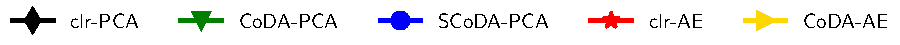
\includegraphics[width=.8\textwidth]{legend}\\%
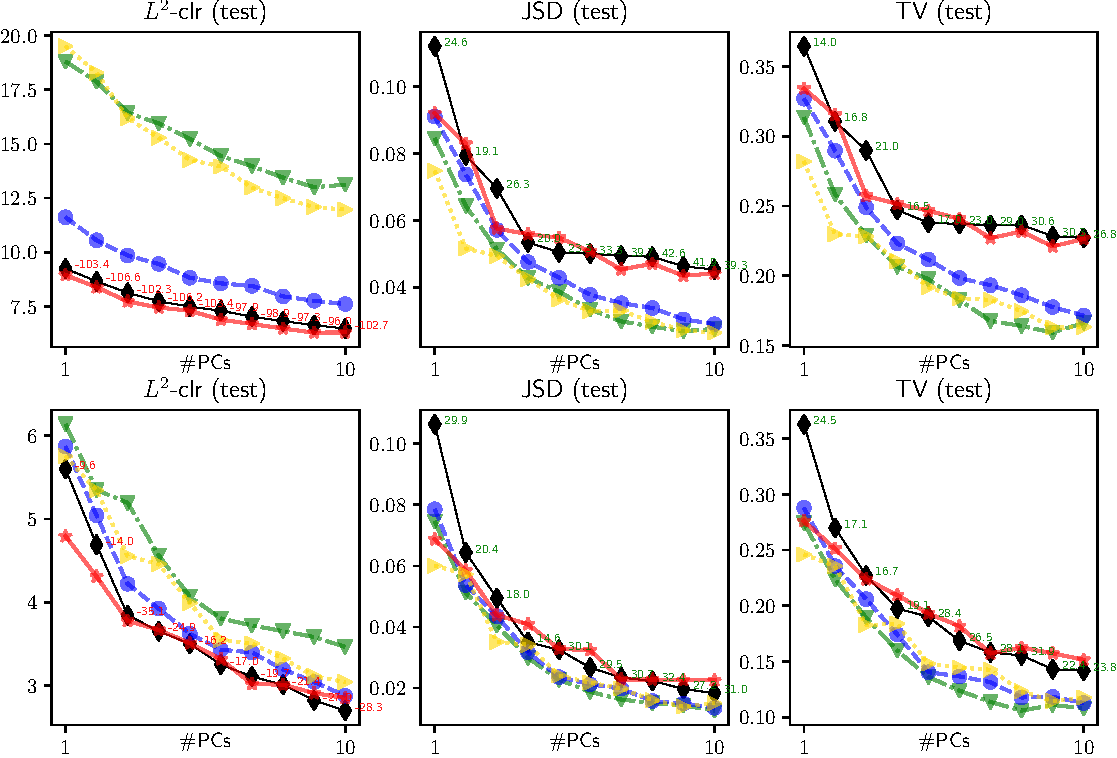
\includegraphics[width=\textwidth]{curves}%
\caption{Testing errors (y-axis) against the number of principal components
(x-axis) based on three different distance measures (from left to right)
on the Atlas data (first row) and the diet swap data (second row).
%The columns, from left to right, show training errors for the HITChip Atlas data,
%corresponding testing errors, training errors for the diet swap data and corresponding test errors.
The numbers along the \texttt{clr-PCA} curves show the percentage of
improvement (green) or disimprovement (red), comparing \texttt{CoDA-PCA} against \texttt{clr-PCA}.\label{fig:result}}
\end{figure}



We compare the following methods:
\texttt{clr-PCA} means PCA applied on the centered log-ratio coordinates;
\texttt{CoDA-PCA} is the proposed \CoDAPCA~in \eqref{pb-CoDA};
\texttt{SCoDA-PCA} is the proposed \surrogateCoDAPCA~in \eqref{pb-s-CoDA};
\texttt{clr-AE} is an autoencoder with $L^2$ loss applied on the clr transformation;
\texttt{CoDA-AE} is the proposed \CoDAAE~in subsection \ref{sec:codaae}.
Both \texttt{clr-AE} and \texttt{CoDA-AE} use
exactly the same structure with one hidden layer of 100 ELU~\cite{cuhFA} units
in their decoders.

The baselines are assessed based on an array of measures including
($L^2$-clr) the $L^2$-distance
$\Vert\clrlog(\bm{x})-\clrlog(\bm{x}')\Vert_{\mathrm{F}}$
between the input data $\bm{x}\in\Se^d$ and the reconstruction $\bm{x}'\in\Se^d$ in the clr space;
(JSD) %normalizing the input and the PCA reconstruction to be probability distributions, then computing
the Jensen-Shannon divergence
$\frac{1}{2}\kl(\bm{x}:\frac{\bm{x}+\bm{x}'}{2})+\frac{1}{2}\kl(\bm{x}':\frac{\bm{x}+\bm{x}'}{2})$;
(TV) the total variation distance $\frac{1}{2}\sum_{i=1}^d\vert{x}_i-{x}'_i\vert$.
These measurements are all invariant to scaling or permutation of $\bm{x}$ and $\bm{x}'$.
See the supplementary material for more baselines and performance indicators.

%\subsection{Microbiome data}

We consider the following datasets available in the microbiome R package~\cite{lsbsMRP},
each of which is randomly split into a training set (90\%) and a testing set (10\%).
%\begin{description}
%  \item A compositional biplot summarizing control and B. fragilis treated microbiomes
%from the \cite{hmhsAMCC} dataset that illustrates the work \cite{gwpeIAR}. There were 10 control (IC) and 10 treated samples (Bf), and 703 OTUs in this dataset. The control and treated samples
%separate poorly for such a small sample set, with 12\% of the variation explained on the
%first principle component, 11\% on the second.
{\emph{The HITChip Atlas dataset \cite{lsssTEI}}} contains 130 genus-level taxonomic groups that
cover the majority of the known bacterial diversity of the human intestine.
The data come from 1006 western adults from 15 western countries (Europe and the United States). Sample sets were analysed with three different DNA extraction methods.
%Visualization of the two main axes of Principal Component Analysis based on the 130 genus-like groups across the 1006 samples.
%While the distribution of samples are clearly related to the DNA extraction method, country differences are not remarkable.
%The second principal axis is driven by the Prevotella group. This broad view is common to most of the PCA methods, however  subtle features differ from one method to another.
{\emph{The two-week diet swap study}} between western (USA) and traditional (rural Africa) diets was reported in \cite{olloFFC}.
In this study, a two-week food exchange was performed in subjects from the same populations, where African Americans were
fed a high-fibre, low-fat African-style diet and rural Africans a high-fat, low-fibre western-style diet.
The group diet was indicated by HE (home environment days), DI (dietary intervention days) and ED (initial and final endoscopy days).
Each subject served as his/her own control, given the known wide individual variation in colonic microbiota composition.

%Visualization of the two main axes of Principal Component Analysis based on the 39 genus-like groups (those encoding the final enzyme in butyrogenesis) across the 223 samples.
%Differences in the microbiota between African Americans and rural Africans are highlighted by visualizing the two main axes of Principal Component Analysis (Americans dominated by genus Bacteroides and Africans by the genus Prevotella).
%Again, this general pattern is common to most of the PCA methods, however, CodaPCA, SCodaPCA and CodaAE provide a clearer picture.

%\item A parallel profiling of gut microbiota versus blood metabolites from \cite{lsksABT} to characterize associations between human intestinal microbiota and blood serum lipids available on the microbiome R package \cite{lsbsMRP}.
%\end{description}

Fig.~\ref{fig:result} shows the typical testing results. We observe
that on most performance indicators \texttt{CoDA-PCA} and \texttt{CoDA-AE}
show a much smaller testing error as compared to \texttt{clr-PCA} and \texttt{clr-AE}, respectively.
The only exception is on $L^2$-clr, where \texttt{clr-PCA} and \texttt{clr-AE}
appear to be favored against our \texttt{CoDA} variants. This is because $L^2$-clr is
exactly the cost function of those two methods.
We found that \texttt{CoDA-AE} is more robust against overfitting as compared to \texttt{clr-AE}.
%Compared with \texttt{CoDA-PCA}, \texttt{CoDA-AE} cannot be easily optimized by a convex
%optimizer and requires more tuning of neural network architecture and learning rates etc.
The performance of \texttt{SCoDA-PCA} is close to \texttt{CoDA-PCA} on most
of the indicators and is better than \texttt{CoDA-PCA} on $L^2$-clr.

%It is clear that on most of the measures %\texttt{CoDA-PCA} and \texttt{CoDA-AE} are favored against the others.
%The exception is the $L^2$-clr figure, where \texttt{clr-PCA} and \texttt{clr-AE} are better. This is because $L^2$-clr is
%exactly the cost function of those two methods.
%where \texttt{CoDA-AE} as a non-linear method is slightly better as it can capture the curvature of the data manifold.
%\subsection{Illustrative Toy Data}

The source codes to reproduce our experimental results are available online\footnote{\url{https://bitbucket.org/RichardNock/coda}}.

\section{Conclusion}

We propose an approach for learning a low dimensional representation
directly on raw count data, which is compositional in nature.
Our proposed algorithm generalizes PCA in two ways, first by going to the exponential
family via the Bregman divergence, and second by converting the normalization of
data to a change in the Bregman divergence. The key theorem used for transforming
the Bregman divergence generalizes a recent result, and may be of independent interest.

\subsection*{Acknowledgements}

The authors gratefully thank Perrine Soret,
Frank Nielsen, Xinhua Zhang, and the anonymous NIPS reviewers,
for their helpful and constructive feedback.
This work was done while MAF was visiting Data61, CSIRO in Canberra, Australia.
%KS is funded by the Investigative Analytics project at Data61.

\bibliography{bibgen}

%include supp in the same tex file for arxiv version
\newpage\appendix%\documentclass{article}

%%% NIPS DEFAULT PACKAGES
%\usepackage{nips_2017}
%\usepackage[utf8]{inputenc} % allow utf-8 input
%\usepackage[T1]{fontenc}    % use 8-bit T1 fonts
%%\usepackage{hyperref}       % hyperlinks
%\usepackage{url}            % simple URL typesetting
%\usepackage{booktabs}       % professional-quality tables
%\usepackage{amsfonts}       % blackboard math symbols
%\usepackage{nicefrac}       % compact symbols for 1/2, etc.
%\usepackage{microtype}      % microtypography

%%% RN stylefile
%\usepackage{morenotations,rotating}
%\usepackage{color,soul,upgreek}
%\usepackage{arydshln}
%\usepackage{wrapfig}
%\usepackage{soul}
%\usepackage{amsmath}
%\usepackage{empheq}
%\usepackage{mdframed,enumerate}


%\usepackage{xr-hyper}
%\externaldocument{nips18-coda-main}

%\usepackage{graphicx}
%\usepackage{caption}
%\usepackage{subcaption}

%%% Tikz Support
%\usepackage{tikz, pgfplots}
%\usetikzlibrary{intersections, calc, positioning, decorations.pathreplacing}
%\pgfplotsset{compat=1.8, xlabel style={anchor=west, align=center}, ylabel style={anchor=south, align=center}, samples=200, ymin=0, ymax=1, width=3cm, height=3cm, axis lines=middle, xticklabel style={/pgf/number format/.cd,frac,frac TeX=\frac}, yticklabel style={/pgf/number format/.cd,frac,frac TeX=\frac}, xtick=\empty,ytick=\empty, no markers, cycle list={{black,solid}}, samples=200}

%\newcommand{\amari}{}

%\title{\papertitle\\(\supplement)}
%%%Adversarial Learning Blurb
%%%How to \st{train} design your $f$-GANs

%%\author{RN}

%\begin{document}

%\maketitle

%\begin{abstract} %This is the supplement for paper "\papertitle".  %\end{abstract}

\addcontentsline{toc}{section}{Appendix}
%\part{Supplementary material on proofs and formal results}
\parttoc

%\section*{\supplement: table of contents}
%\noindent \textbf{Supplementary material on proofs and formal results}
%\hrulefill Pg \pageref{the_theo}\\
%\noindent Proof of Theorem \ref{thCODA1}\hrulefill Pg
  %\pageref{sec-proof-thCODA1}\\
%\noindent Proof of Lemma \ref{lemMU}\hrulefill Pg
  %\pageref{sec-proof-lemMU}\\
%\noindent Proof of Lemma \ref{lemHESS}\hrulefill Pg
  %\pageref{sec-proof-lemHESS}\\

%\noindent \textbf{Supplementary material on experiments} \hrulefill
%Pg \pageref{exp_expes}\\


\newpage

\section{Convexity of divergence}

\begin{theorem}\label{thCODA1}
For any $\A$, $\V$ such that $\A^\top \V \ve{1} = \ve{0}$, letting $D_{\exp}$ the Bregman divergence with generator
$\varphi^\star(z) \defeq \exp z$ and $\kl$ the generator for KL
divergence,
\begin{eqnarray}
 D_{\exp}(\V^\top
\ve{a}_i\|\clrlog({\ve{x}_i}))  & = &  q_i \cdot D_{\check{\kl}} (\ve{x}_i \|
\exp(\V^\top \ve{a}_i)) + r_i \cdot D_{g}(\ve{x}_i
\| \exp(\V^\top \ve{a}_i)), \forall i = 1, 2, ..., m\:\:,
\end{eqnarray}
with $q_i \defeq 1/g(\ve{x}_i)$ and $r_i \defeq q_i \cdot \sum_j
\exp\left(\ve{a}^\top_i
      \ve{v}_j\right)$, satisfying $r_i \geq d q_i$.
\end{theorem}
(Proof in \SM, Section \ref{sec-proof-thCODA1})

We can remark that
\begin{eqnarray}
\frac{1}{g(\ve{x}_i)} \cdot \sum_j
\exp\left(\ve{a}^\top_i
      \ve{v}_j\right) & = & \sum_j
\exp\left(\ve{a}^\top_i
      \ve{v}_j - x_{ij}\right) \check{x}_{ij}.
\end{eqnarray}

To generalize the notion of geometric average, consider any strictly convex function
$\varphi : \mathbb{R} \rightarrow \mathbb{R}$ at least three times
differentiable and with invertible derivative. Define the
$\varphi$-mean of $\ve{x}$ as
\begin{eqnarray}
\mu_{\varphi}(\ve{x}) & \defeq & \varphi'^{-1}\left(\E_i \varphi'(x_i)\right).
\end{eqnarray}
We now state a Lemma which will be essentially used for a particular
case of $\varphi$ but may be of independent interest for more general
cases, as explained in the following examples.
\begin{lemma}\label{lemMU}
Let $\varphi$ convex and at least three times differentiable. Let
\begin{eqnarray}
\phi(x) & \defeq & -\frac{\varphi'''(x)}{(\varphi''(x))^2}\:\:.
\end{eqnarray}
Then the $\varphi'$-mean $\mu_\varphi$ is convex (resp. concave) iff
\begin{eqnarray}
\phi(\mu_\varphi(\ve{x}))& \geq \mbox{ (resp. $\leq$)}& m \cdot \min_i
\phi(x_i) \:\:, \forall \ve{x}\:\:. \label{eqCONDNS}
\end{eqnarray}
\end{lemma}
(Proof in \SM, Section \ref{sec-proof-lemMU})
\begin{example}\label{exGEOM}
Take for example $F'(x) \defeq \ln x$ (geometric average). In this
case, $\phi(x) = +1$ and ineq. (\ref{eqCONDNS}) brings $1 \leq m$ for
the concavity of the mean and shows that $g$ is concave.
\end{example}
\begin{example}
Consider $F'(x) = -1/x$ (harmonic
average, over $\mathbb{R}_+$). In this case, $\phi(x) = + x$, so to prove the concavity of
the mean, we need to show $\mu_F(\ve{x}) \leq m \min_i x_i$, which is
equivalent to show
\begin{eqnarray}
\sum_i \frac{1}{x_i} & \geq & \max_i \frac{1}{x_i}\:\:,
\end{eqnarray}
and shows the concavity of the mean.
\end{example}
\begin{example}
Consider $F' = \exp$ (normalized
softmax). In this case, $\phi(x) = -\exp(-x)$, which shows that the
mean cannot be concave. To show its convexity, we need to show
equivalently
\begin{eqnarray}
\frac{1}{\sum_i \exp x_i} & \leq & \exp( - \max_i x_i)\:\:,
\end{eqnarray}
which is equivalent to $\sum_i \exp(x_i - \max_j x_j) \geq 1$, and
because of the non-negativity of the exponential,
shows the convexity of the mean.
\end{example}


\section{Proof of Theorem \ref{thCODA1}}\label{sec-proof-thCODA1}

First,
letting $\ve{y}_i \defeq \exp(\V^\top \ve{a}_i)$ for any $i = 1, 2, ...,
m$, and $\ve{v}_j$ the $j$-th row of $\V$ (as a column vector), we get
\begin{eqnarray}
\varphi^\star\left(\nabla\varphi(\veydagger_i)\right) & = & \sum_j
\exp\left( \log \left( \exp\left( \ve{a}^\top_i
      \ve{v}_j\right)\right)\right) = \sum_j
\exp\left(\ve{a}^\top_i
      \ve{v}_j\right)\label{eq1}.
\end{eqnarray}
We recall $g(\ve{x}) =
(\prod_k x_k)^{1/d}$, the geometric mean. So,
\begin{eqnarray}
g(\exp(\V^\top \ve{a}_i)) & = & \exp\left(\frac{1}{d} \sum_j \ve{a}^\top_i
      \ve{v}_j\right) = \exp((\A^\top \V \ve{1})_i) = \exp(0) = 1,
\end{eqnarray}
because of the constraint $\A^\top \V \ve{1} = \ve{0}_m$. Hence,
letting $\ve{y}_i \defeq \exp(\V^\top \ve{a}_i)$ for short, we obtain
$\check{\ve{y}}_i = \ve{y}_i$. Also, the dual symmetry of Bregman
divergences \citep{bnnBV} yields:
\begin{eqnarray}
D_{\exp}(\V^\top \ve{a}_i \|\clrlog({\ve{x}_i})) & = & D_{\kl} (\check{\ve{x}}_i \|
\exp(\V^\top \ve{a}_i))\:\:.
\end{eqnarray}
We now use Theorem \ref{th00}. It comes (letting again $\ve{y}_i \defeq \exp(\V^\top \ve{a}_i)$ for
short) that for any $i=1, 2, ..., m$,
\begin{align}
&g(\ve{x}_i) \cdot D_{\exp}(\V^\top \ve{a}_i\|\clrlog({\ve{x}_i}))\nonumber\\
=\;&   g(\ve{x}_i) \cdot D_{\kl} (\check{\ve{x}}_i \|
\exp(\V^\top \ve{a}_i))\nonumber\\
=\;&  D_{\check{\kl}}\left( \ve{x}_i \bigm\|
  \exp(\V^\top \ve{a}_i)\right) +
\varphi^\star\left(\nabla\varphi(\veydagger_i)\right) D_{g}(\ve{x}_i
\| \ve{y}_i)\nonumber\\
=\;&  D_{\check{\kl}}\left( \ve{x}_i \bigm\|
  \exp(\V^\top \ve{a}_i)\right) +
\left(\sum_j
\exp\left(\ve{a}^\top_i
      \ve{v}_j\right)\right)\cdot D_{g}(\ve{x}_i
\| \exp(\V^\top \ve{a}_i))\:\:,
\end{align}
which brings the statement of the Theorem. The fact that $r_i \geq d
q_i$ follows from the convexity of $\exp$.

\section{Proof of Lemma \ref{lemMU}}\label{sec-proof-lemMU}

Let $\mu_\varphi(\ve{x}) \defeq \varphi'^{-1}((1/m)\cdot \sum_i
\varphi'(x_i))$ the $\varphi'$-mean of the coordinates of
$\ve{x}$. Then
\begin{eqnarray}
\frac{\partial}{\partial x_i} \mu_\varphi(\ve{x}) & = &
\frac{1}{m}\cdot
\frac{\varphi''(x_i)}{\varphi''(\mu_\varphi(\ve{x}))}\:\:,\\
\frac{\partial^2}{\partial x_i \partial x_j} \mu_\varphi(\ve{x}) & = &
\frac{1}{m \varphi''(\mu_\varphi(\ve{x}))}\cdot \left(\delta_{ij}\cdot
  \varphi'''(x_i)-
  \frac{\varphi'''(\mu_\varphi(\ve{x}))}{m (\varphi''(\mu_\varphi(\ve{x})))^2}\cdot
  \varphi''(x_i) \varphi''(x_j)\right)
\end{eqnarray}
$\ve{x}$ being fixed, let $\tilde{\ve{y}}$ the vector defined by $\tilde{y}_i \defeq y_i
\cdot \varphi''(x_i)$ and let
\begin{eqnarray}
\phi(x) & \defeq & -\frac{\varphi'''(x)}{(\varphi''(x))^2}\:\:.
\end{eqnarray}
Let $\Phi$ the diagonal matrix with
$\Phi_{ii} \defeq \phi(x_i)$. The Hessian $\matrice{h}_{\mu_\varphi(\ve{x})}$ satisfies
\begin{eqnarray}
\ve{y}^\top \matrice{h}_{\mu_\varphi(\ve{x})} \ve{y} & = & \frac{1}{m
  \varphi''(\mu_\varphi(\ve{x}))}\cdot
\left(\frac{\phi(\mu_\varphi(\ve{x}))}{m}\cdot \tilde{\ve{y}}^\top
  \tilde{\ve{y}} - \tilde{\ve{y}}^\top
  \Phi \tilde{\ve{y}} \right)\nonumber\\
 & = & \frac{1}{m
  \varphi''(\mu_\varphi(\ve{x}))}\cdot
\tilde{\ve{y}}^\top \mathrm{Diag}\left(
  \frac{\phi(\mu_\varphi(\ve{x}))}{m}\cdot \ve{1} - \ve{\phi}(\ve{x})\right) \tilde{\ve{y}}
\end{eqnarray}
We see that when $\varphi''$ is
not zero everywhere, $\tilde{\ve{y}}$ spans the same set as $\ve{y}$,
so if $\varphi$ is convex, $\mu_\varphi$ is
convex iff
$(\phi(\mu_\varphi(\ve{x}))/m)\cdot \ve{1} - \ve{\phi}(\ve{x})
\geq \ve{0}$, that is
\begin{eqnarray}
\phi(\mu_\varphi(\ve{x}))& \geq & m \cdot \phi(x_i)\:\:, \forall i\:\:,
\end{eqnarray}
which is equivalent to the Lemma's statement.

%\section{Proof of Theorem \ref{thmSMOOTH}}
%We extend the definition of the geometric mean to $\Se\cup\partial\Se$ so that
%$g(\ve{x})=\prod_{j:x_j>0} x_j^{1/d^+}$, where
%$d^+=\vert\{j\,:\,x_j>0\}\vert$. In this way $\check{\ve{x}}$ is defined
%as a continuous function on the whole manifold with boundary. This is only a
%technical treatment as we assume $\ve{x}$ is given.

%By noting that $\exp(\clrlog(\ve{x}))=\check{\ve{x}}$, we have
%\begin{align}
%D_{\exp}(\ve{y}\,\Vert\,\clrlog(\ve{x}))
%&=
%\bm{1}^\top\bigg[ \exp(\ve{y}) - \check{\ve{x}} - \check{\ve{x}}\circ\left(\ve{y}-\clrlog(\ve{x})\right) \bigg]\nonumber\\
%&=
%\bm{1}^\top\exp(\ve{y}) - \check{\ve{x}}^\top \ve{y} +
%\mathrm{constant}\nonumber\\
%&=
%\sum_j \exp(y_j) - \sum_{j:x_j>0} \check{x}_j^\top y_j +
%\mathrm{constant}
%\end{align}
%Note that the coordinate cart $(y_1,y_2,\cdots)$
%only covers the interior of the plane $\ve{1}^\top\ve{y}=0$
%but cannot cover its boundary.
%On the boundary (where $y_j=-\infty$) we have to change the chart to $z_j=\exp(y_j)$.
%In this case the function becomes 
%\begin{align}
%D_{\exp}(\ve{y}\,\Vert\,\clrlog(\ve{x}))
%=\sum_j z_j - \sum_{j:x_j>0} \check{x}_j^\top \log{z}_j,
%\end{align}
%which is a smooth function near the boundary when $z_j=0$ and $x_j=0$.

\section{Proof of Lemma \ref{lemHESS}}\label{sec-proof-lemHESS}

We have
\begin{eqnarray}
\check{\kl}(\ve{x}) & = & \left(\sum_i x_i\log x_i - x_i\right) - \frac{1}{d}
\cdot \sum_{ij} x_i \log x_j
\:\:,\\
\frac{\partial}{\partial x_i} \check{\kl}(\ve{x}) & = & \log x_i -
\frac{1}{d} \cdot \sum_j \log x_j -\frac{1}{d x_i} \cdot \sum_j x_j
\\
 & = & -\frac{1}{d}\cdot \left(\sum_j \frac{x_j}{x_i} + \log \frac{x_j}{x_i} \right)\:\:,\label{eq:grad}\\
\frac{\partial^2}{\partial x_i \partial x_j} \check{\kl}(\ve{x}) & = &
-\frac{1}{d} \cdot \left( \frac{1}{x_i} + \frac{1}{x_j} \right), \forall j\neq i,\\
\frac{\partial^2}{\partial x_i^2} \check{\kl}(\ve{x}) & = &
\frac{1}{x_i}\cdot \left( 1 - \frac{1}{d} + \frac{1}{d}\cdot
  \sum_{j\neq i}\frac{x_j}{x_i}\right).
\end{eqnarray}
We then check that
\begin{eqnarray}
(\hessian \ve{z})_i & = & \frac{z_i}{x_i} + \frac{1}{d} \cdot \sum_j
\left(\frac{z_i x_j}{x_i^2} - \frac{z_j}{x_j} - \frac{z_j}{x_i}\right)
\end{eqnarray}
and finally
\begin{eqnarray}
\ve{z}^\top \hessian \ve{z} & = & \sum_i \frac{z^2_i}{x_i} +
\frac{1}{d}\sum_{ij}\left(\frac{z_i^2x_j}{x_i^2} - \frac{z_iz_j}{x_j}
  - \frac{z_i z_j}{x_i}\right) \nonumber\\
 & = & \frac{1}{d}\sum_{ij}\left(\frac{z_i^2x_i}{x_i^2} + \frac{z_i^2x_j}{x_i^2} - \frac{z_iz_j}{x_j}
  - \frac{z_i z_j}{x_i}\right) \nonumber\\
 & = & \frac{1}{d}\sum_{ij}\left(\frac{z_i^2x_ix_j^2 + z_i^2x_j^3-z_iz_jx_i^2x_j-z_iz_jx_ix_j^2}{x_i^2x_j^2}\right) \nonumber\\
 & = & \frac{1}{2d}\sum_{ij}\left(\frac{z_i^2x_ix_j^2 + z_i^2x_j^3+z_j^2x^2_ix_j + z_j^2x_i^3-2z_iz_jx_i^2x_j-2z_iz_jx_ix_j^2}{x_i^2x_j^2}\right) \nonumber\\
 & = & \frac{1}{2d}\sum_{ij}\left(\frac{z_i^2x_j^2(x_i+x_j) + z_j^2x^2_i(x_i+x_j) -2z_iz_jx_ix_j(x_i+x_j)}{x_i^2x_j^2}\right) \nonumber\\
 & = & \frac{1}{2d}\sum_{ij}(x_i+x_j)\cdot \left(\frac{z_i}{x_i}-\frac{z_j}{x_j}\right)^2,
\end{eqnarray}
as claimed. This also shows the convexity of $\check{\kl}(\ve{x})$.

We now show that $\check{\kl}
\circ \exp$ is
1-homogeneous on the subspace $\mathrm{span}(\{\ve{1}\})^\bot$, which
means, by Euler's Theorem,
\begin{eqnarray}
\check{\kl}(\exp(\ve{x})) & = & \exp(\ve{x})^\top \nabla
\check{\kl}(\exp(\ve{x})), \forall \ve{x}\in \mathrm{span}(\{\ve{1}\})^\bot.
\end{eqnarray}
To see this, we write
\begin{eqnarray}
\lefteqn{\check{\kl}(\exp(\ve{x})) - \exp(\ve{x})^\top \nabla \check{\kl}(\exp(\ve{x}))}\nonumber\\
 & = & \sum_j x_j \exp(x_j) -
 \exp(x_j) \nonumber\\
 & & +\frac{1}{d} \cdot \sum_j \left(
   \exp(x_j)\cdot \sum_k \left( \exp(x_k - x_j) + (x_k - x_j)\right) \right) \nonumber\\
 & = & \sum_j x_j \exp(x_j) \underbrace{-
 \sum_j \exp(x_j) + \sum_k  \exp(x_k)}_{=0} \nonumber\\
 & & + \frac{1}{d}\cdot \sum_{j} \exp(x_j) \underbrace{\sum_k x_k}_{=0} - \sum_{j} \exp(x_j) x_j \nonumber\\
 & = & \sum_j x_j \exp(x_j) - \sum_{j} \exp(x_j) x_j \nonumber\\
 & = & 0,
\end{eqnarray}
where we have used the fact that $\ve{1}^\top \ve{x} = 0$.

\section{Derivations of the unconstrained optimization in
\eqref{eq:unconstrainedcoda} and \eqref{eq:unconstrainedscoda}}

Consider that $\X$ is constant, therefore
\begin{align*}
\ell_{\mathrm{CoDA\text{-}PCA}}(\X; \A, \V)
=\:& D_{\exp}(\V^\top\A\,\Vert\, \clrlog({\X}))\nonumber\\
=\:&
\bm{1}^\top
\bigg[
\exp(\V^\top\A) - \exp(\clrlog({\X})) - (\V^\top\A - \clrlog({\X}))\circ\exp(\clrlog({\X}))
\bigg]\bm{1}\nonumber\\
=\:&
\bm{1}^\top
\bigg[
\exp(\V^\top\A) - \V^\top\A\circ\exp(\clrlog({\X}))
\bigg]\bm{1} + \mathrm{constant}\nonumber\\
=\:&
\bm{1}^\top
\bigg[
\exp(\V^\top\A) - \V^\top\A\circ\check{\X}
\bigg]\bm{1} + \mathrm{constant}.
\end{align*}
Let $\Y=\V^\top\A$, and we get \eqref{eq:unconstrainedcoda}.

By \eqref{eq:grad}, if $\bm{y}_i$ is centered and $\bm{y}_i^\top\bm{1}=0$, we have
\begin{align*}
\bigtriangledown \check{\kl}( \exp(\bm{y}_i) )
&= -\frac{1}{d}\cdot \left[\exp(\bm{1}\bm{y}_i^\top - \bm{y}_i\bm{1}^\top)
+ \bm{1}\bm{y}_i^\top - \bm{y}_i\bm{1}^\top \right]\bm{1}\nonumber\\
&= -\frac{1}{d} \exp(\bm{1}\bm{y}_i^\top - \bm{y}_i\bm{1}^\top) \bm{1} + \bm{y}_i.
\end{align*}
Therefore
\begin{align*}
\ell_{\surrogateCoDAPCA}(\X; \A, \V)
&=\sum_i \left[ \check{\bm{x}}_i^\top
\frac{1}{d}
\exp(\bm{1}\bm{y}_i^\top - \bm{y}_i\bm{1}^\top)
\bm{1} - \check{\bm{x}}_i^\top \bm{y}_i \right]\nonumber\\
&=\sum_{i} \check{\bm{x}}_i^\top
\left[\exp(-\bm{y}_i) \exp(\bm{y}_i^\top)\frac{\bm{1}}{d}
- \bm{y}_i\right],
\end{align*}
which, in matrix form, is \eqref{eq:unconstrainedscoda}.

\section{More Experimental Results}

We include another baseline \texttt{CoDA-PCA}$^*$ that is the
non-parametric version of \texttt{CoDA-PCA} optimized by L-BFGS.
Note that \texttt{CoDA-PCA}$^*$ does not learn an encoding map
and therefore cannot provide an out-of-sample extension.

The baselines are further assessed based on 
(symmetric perspective KL divergence; SPKL) normalizing
the geometric average of the input data $p$ and
the PCA reconstruction $q$ and get respectively
two positive measures $\check{p}$ and $\check{q}$, then computing the
symmetric KL divergence
$\frac{1}{2}\sum_{i}\left(\check{p}_i\log\frac{\check{p}_i}{\check{q}_i}+\check{q}_i\log\frac{\check{q}_i}{\check{p}_i}\right)$;
($L^2$) $L^2$-distance of $\bar{p}$ and $\bar{q}$ after the normalizing $p$ and
$q$ into the probability simplex.
(Riemannian) the Riemannian distance between the two probabilities
$\bar{p}$ and $\bar{q}$ defined by the Fisher information metric, given by
$2\arccos\left(\sqrt{\bar{p}}^\top\sqrt{\bar{q}}\right)$.

Fig.~\ref{fig:fullresult} shows the training and testing errors.
A key observation is that 
\texttt{CoDA-PCA}$^*$ is slightly better than \texttt{CoDA-PCA}
because the embedding points are free parameters 
and are not constrained by a neural network.
We also see that
\texttt{clr-AE} shows small training errors but does not
generalize as well as \texttt{CoDA-AE} on the testing set.

\begin{figure}[!t]
\centering
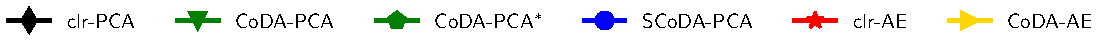
\includegraphics[width=\textwidth]{legend_ext}\\%
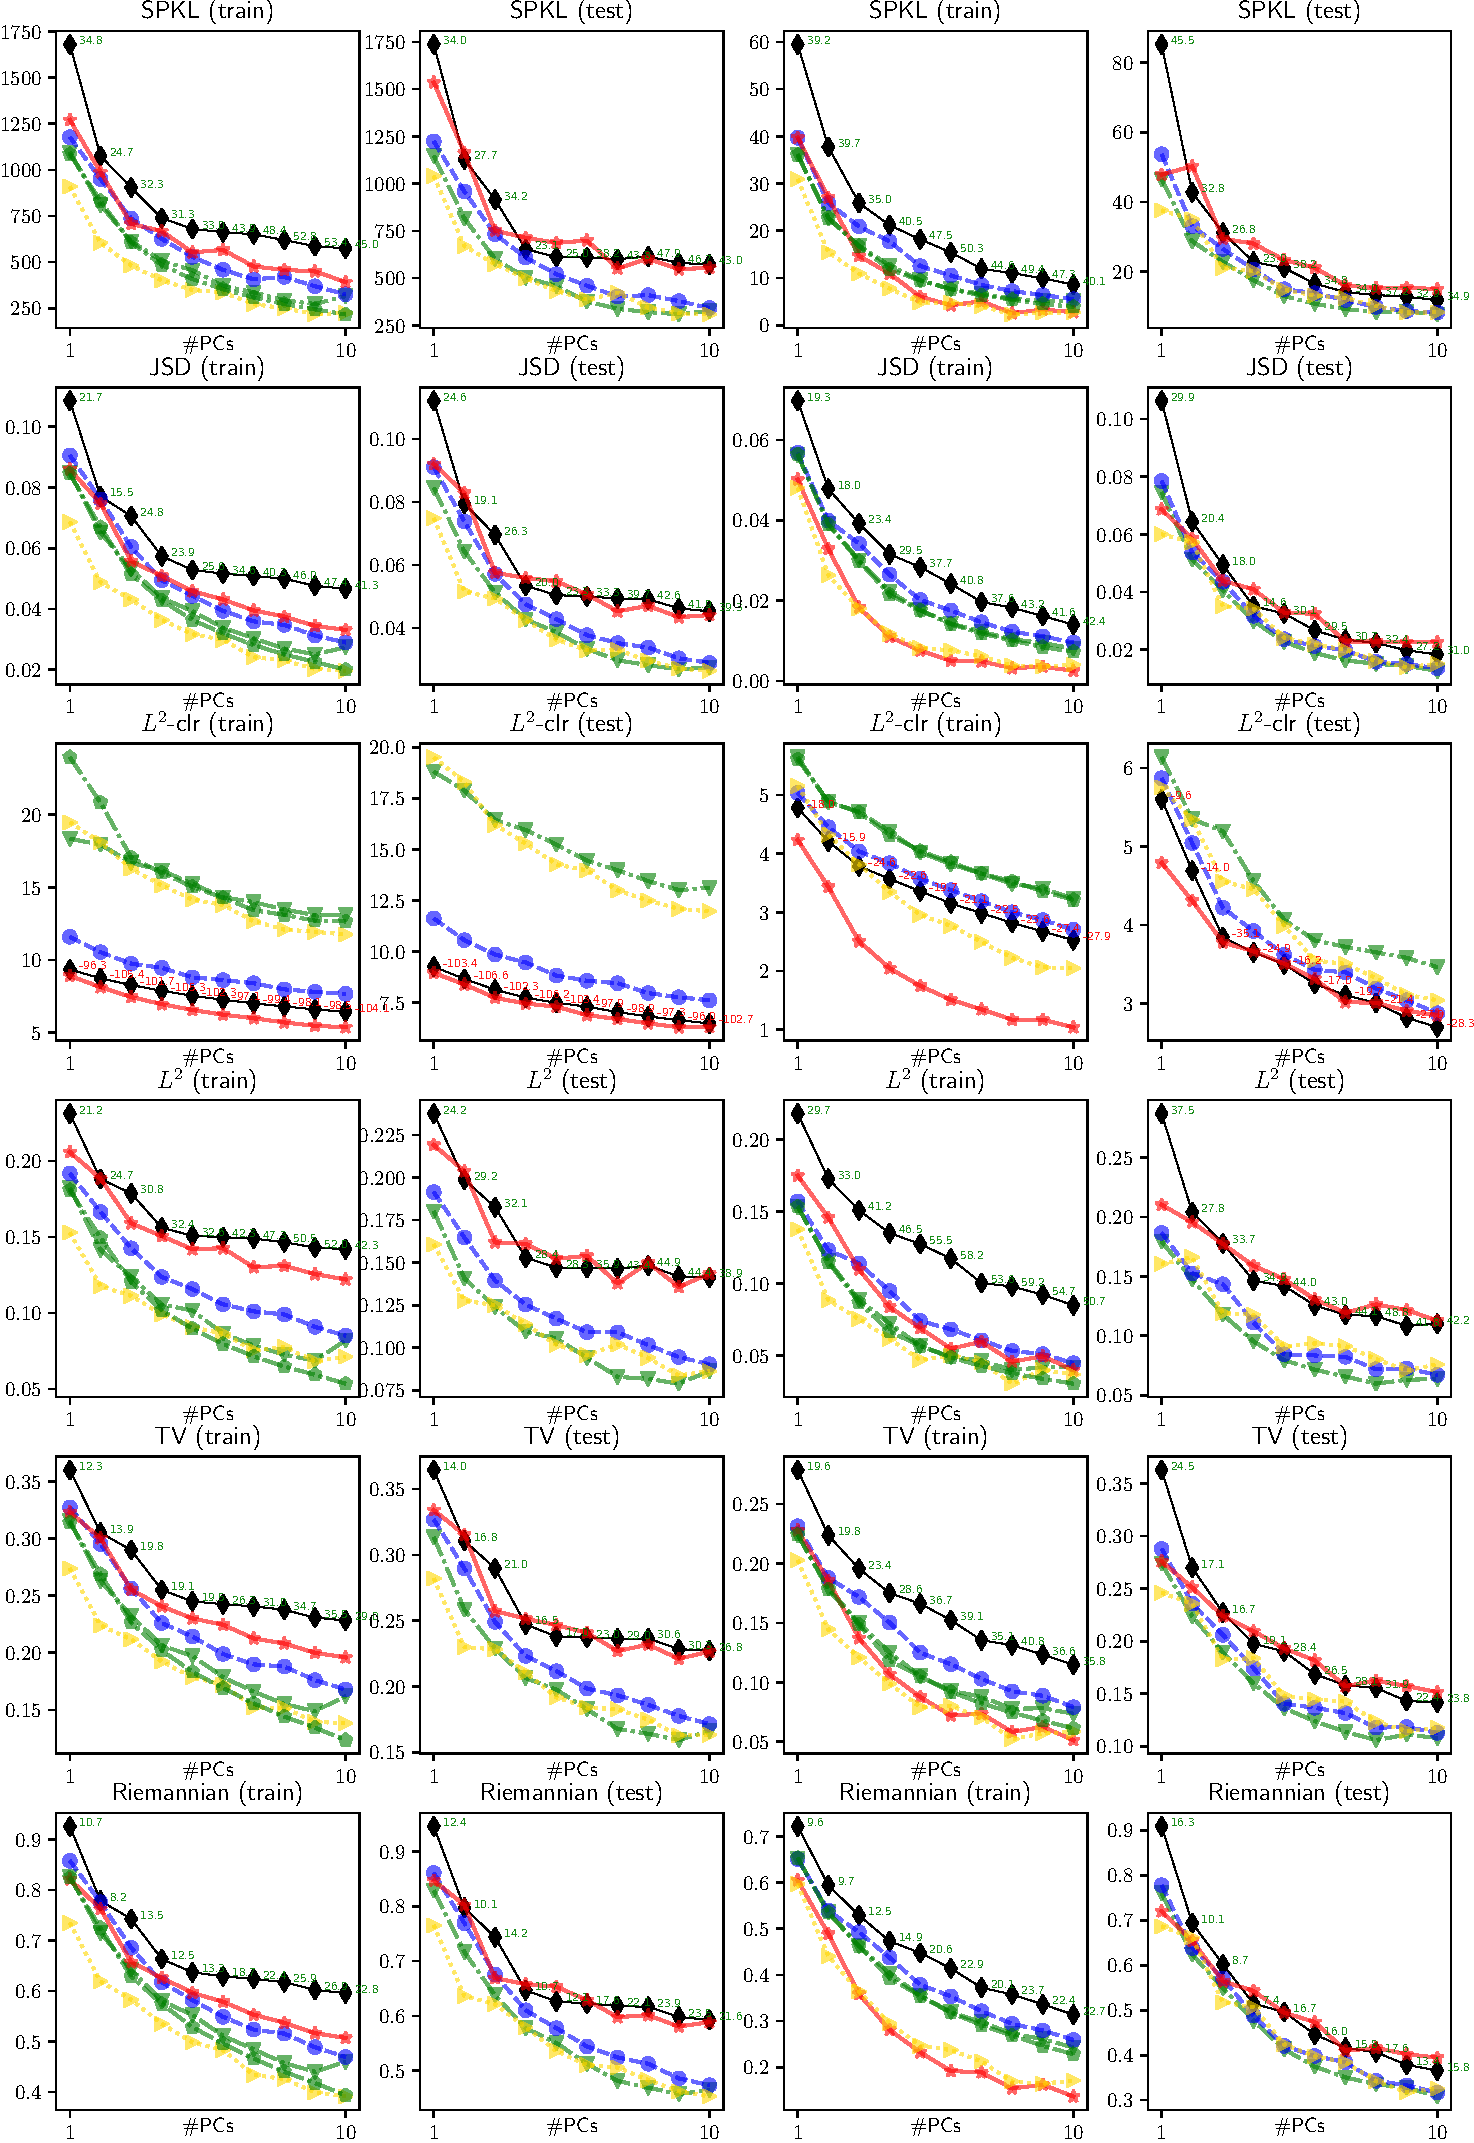
\includegraphics[width=\textwidth]{fullcurves}%
\caption{Training and testing errors measured by different distances
against the number of principal components.
The columns, from left to right, show training errors (Atlas),
corresponding testing errors, training errors (diet swap) and corresponding test errors.\label{fig:fullresult}}
\end{figure}




%\bibliographystyle{plain}
%\bibliography{bibgen}

%\end{document}


\end{document}
